\documentclass[a4paper]{article}

\usepackage[T2A]{fontenc}
\usepackage[russian]{babel}
\usepackage{graphicx}
\usepackage{float}
\usepackage{hyperref}
\usepackage{amsmath, amssymb, diffcoeff, mathtools}
\usepackage{caption}
\usepackage{geometry}
\usepackage{pdfpages}
\usepackage{wrapfig}

\begin{document}

\begin{center}
\textsc{Санкт-Петербургский национальный исследовательский институт информационных технологий, механики и оптики\\[3mm]
Физический факультет} \\[3mm]

\end{center}
\vspace{5mm}
\line(1,0){\textwidth}
\begin{center}
\textbf{ЛАБОРАТОРНАЯ РАБОТА №2.3\\}
\textbf{"Определение показателя адиабаты методом стоячих волн"}
\end{center}
\vspace{2mm}
\line(1,0){\textwidth}
\vspace{5mm}
\begin{minipage}{0.4\textwidth}
    Группа: Z3144 \\
    Студент: Турчанин Евгений\\
    \vspace{1mm}
\end{minipage}
\hfill
\vspace{1mm}
\line(1,0){\textwidth}

\subsection*{Цель работы}
1. Определение показателя адиабаты для воздуха при комнатной температуре.

\subsection*{Задачи}
1. Прямое измерение координат пучностей стоячей волны в трубке, частично заполненной водой.

2. Определение скорости звука в воздухе.

\subsection*{Введение}
Количество теплоты, необходимое для изменения температуры массы $m$ некоторого вещества на величину $\Delta T$, определяется соотношением
\[
\Delta Q = C \frac{m}{\mu} \Delta T
\]
(1)

где величина $C$ называется молярной теплоемкостью. Для газа теплоемкость существенно зависит от условий нагревания. Это связано с тем, что часть подводимой к нему теплоты может расходоваться на работу, совершаемую при расширении газа. Важную роль в теории идеального газа имеет показатель адиабаты:
\[
\gamma = \frac{C_p}{C_v}
\]
(2)

Здесь $C_p$ и $C_v$ — теплоемкости газа при постоянном давлении и постоянном объеме, соответственно. Можно показать, что если не возбуждены колебания молекулы, то
\[
\gamma = \frac{i + 2}{i}
\]
(3)

\subsection*{}
где $i$ — число степеней свободы молекулы. В частности, для одноатомного газа $i = 3$, для двухатомного — $i = 5/2$.

Экспериментально величину $\gamma$ можно определить на основе скорости распространения звуковых волн в газе. При распространении звука происходит сжатие и расширение газа. Поскольку эти процессы при частоте порядка $10^3 \, \text{Гц}$ протекают очень быстро, то теплообмен между различными областями звуковой волны отсутствует. Процессы такого типа называются адиабатическими. Для идеального газа адиабатические процессы описываются уравнением
\[
pV^\gamma = \text{const}
\]

Как следствие, скорость звука в газе зависит от коэффициента $\gamma$, и вычисляется по формуле
\[
v = \sqrt{\frac{RT\gamma}{\mu}}
\]
(5)

где $T$ — абсолютная температура; $\mu$ — молярная масса газа, $R = 8,31 \, \text{Дж/К·моль}$ — универсальная газовая постоянная.

В данной работе скорость звука измеряется косвенным образом на основе длины волны звуковых стоячих волн. Волны такого типа обычно образуются при отражении обычной бегущей волны от препятствий.

Отклонение давления газа от равновесного значения в плоской стоячей волны зависит от координаты $x$ и времени $t$ по формуле
\[
\Delta p(x,t) = A_m \cos \left( \frac{2\pi x}{\lambda} \right) \cos (\omega t)
\]
(6)

где $A_m$ — амплитуда; $\lambda$ — длина волны; $\omega$ — циклическая частота. В каждой точке $x$ такой волны величина $\Delta p$ гармонически колеб-

\subsection*{}
дется с частотой $\nu = \omega/2\pi$. При этом амплитуда колебаний при

изменении координаты $x$ периодически меняется в пространстве

от 0 до максимального значения $A_m$.

Области, где амплитуда максимальная, называются пучностя-
ми волны, а точки, где колебания отсутствуют, — узлами. Из (6)

следует, что расстояние между соседними пучностями или узлами

равно
\[
l = \frac{\lambda}{2}
\]
\section{Экспериментальная установка}

Стоячие волны исследуются на установке, представленной на
Рис. 1.

\begin{figure}[H]
    \begin{center}
        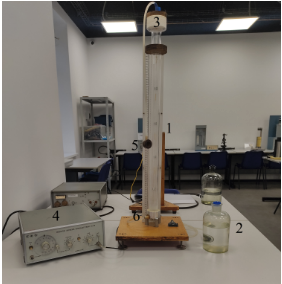
\includegraphics[width=0.6\textwidth]{fig_1}
        \caption{Внешний вид экспериментальной установки}
    \end{center}
\end{figure}


\begin{figure}[H]
    \begin{center}
        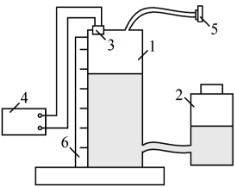
\includegraphics[width=0.6\textwidth]{fig_2}
        \caption{Схема установки}
    \end{center}
\end{figure}

Стоячая звуковая волна образуется в цилиндрической стеклянной трубке 1, частично заполненной водой. Уровень воды можно изменять, поднимая и опуская сосуд 2. Источником звука является микрофон 3, на который подается синусоидальное напряжение от звукового генератора 4. Уровень громкости звука
определяется на слух с помощью наушника 5, соединенного резиновой трубкой с воздухом в цилиндре. Положение уровня воды
измеряется по шкале 6.\\
Звуковая волна распространяется вдоль цилиндра и отражается от поверхности воды. В результате в трубе возникает ряд
пучностей, характерных для стоячей воды. Отметим, что полного
отсутствия колебаний в узлах не наблюдается, что можно объяснить различием амплитуд падающих и отраженных волн.\\
Изменение уровня воды в цилиндре вызывает смещение стоячей волны, поскольку один из узлов находится на поверхности
жидкости. Как следствие, изменяется и громкость звука, воспринимаемого через наушник. Согласно формуле (7), расстояние
между уровнями воды, соответствующими соседним максимумам
громкости, составляет $\lambda/2$. Определив расстояние между соседними уровнями воды, при которых наблюдается максимум громкости звука в наушнике, находят длину волны $\lambda$. Исходя из частоты $\nu$ звука и длины волны, вычисляется скорость звука:
\begin{equation}
    v = \lambda \nu
\end{equation}
По известной температуре и скорости звука, с помощью соотношения (5) , можно найти показатель адиабаты 𝛾.


\section{Обработка результатов}
\subsection{Расчёт средних значений координат и расстояний между пучностями}
Средние координаты пучностей \( \langle X_i \rangle \) и расстояния между ними \( l_i \) рассчитаны по формулам:
\[
\langle X_i \rangle = \frac{1}{N} \sum_{k=1}^N X_{i,k}, \quad l_i = \langle X_{i+1} \rangle - \langle X_i \rangle
\]
где \( N = 5 \) — количество измерений. Результаты представлены в таблице:

\begin{table}[h!]
\centering
\caption{Результаты измерений и расчётов}
\begin{tabular}{|c|c|c|c|c|c|}
\hline
П.П. & \( X_1 \), м & \( X_2 \), м & \( X_3 \), м & \( X_4 \), м & \( X_5 \), м \\ \hline
1 & 0.118 & 0.224 & 0.341 & 0.472 & 0.581 \\ \hline
2 & 0.115 & 0.227 & 0.337 & 0.471 & 0.586 \\ \hline
3 & 0.120 & 0.235 & 0.348 & 0.475 & 0.583 \\ \hline
4 & 0.118 & 0.226 & 0.344 & 0.463 & 0.570 \\ \hline
5 & 0.113 & 0.230 & 0.342 & 0.468 & 0.572 \\ \hline
\multicolumn{6}{c}{} \\[-0.5em]
\hline
\( \langle X_i \rangle \), м & 0.1168 & 0.2284 & 0.3424 & 0.4698 & 0.5784 \\ \hline
\( l_i \), м & 0.1116 & 0.1140 & 0.1274 & 0.1086 & — \\ \hline
\end{tabular}
\end{table}

Среднее расстояние между пучностями:
\[
l = \frac{1}{4} \sum_{i=1}^4 l_i = \frac{0.1116 + 0.1140 + 0.1274 + 0.1086}{4} = 0.1154 \, \text{м}
\]

\subsection{Расчёт скорости звука}
Скорость звука вычислена по формуле:
\[
v = 2 \cdot l \cdot \nu = 2 \cdot 0.1154 \, \text{м} \cdot 1500 \, \text{Гц} = 346.2 \, \text{м/с}
\]

\subsection{Определение показателя адиабаты}
Используя формулу для скорости звука \( v = \sqrt{\frac{R T \gamma}{\mu}} \), выразим \( \gamma \):
\[
\gamma = \frac{v^2 \mu}{R T} = \frac{(346.2)^2 \cdot 0.029}{8.314 \cdot 298} = 1.39
\]
Теоретическое значение для воздуха (\( i = 5 \)):
\[
\gamma_{\text{теор}} = \frac{i + 2}{i} = \frac{5 + 2}{5} = 1.4
\]

\subsection{Анализ погрешностей}
Погрешность \( \gamma \) рассчитана методом линеаризации:
\[
\delta \gamma = \gamma \sqrt{\left(2 \frac{\delta l}{l}\right)^2 + \left(\frac{\delta \nu}{\nu}\right)^2 + \left(\frac{\delta T}{T}\right)^2}
\]
При \( \delta l = 0.002 \, \text{м} \), \( \delta \nu = 10 \, \text{Гц} \), \( \delta T = 1 \, \text{К} \):
\[
\delta \gamma = 1.39 \sqrt{\left(2 \cdot \frac{0.002}{0.1154}\right)^2 + \left(\frac{10}{1500}\right)^2 + \left(\frac{1}{298}\right)^2} \approx 0.04
\]
Окончательный результат:
\[
\gamma = 1.39 \pm 0.04, \quad \gamma_{\text{теор}} = 1.40
\]

\subsection{Выводы}
В ходе проведения эксперимента Экспериментальное значение \( \gamma = 1.39 \pm 0.04 \) совпадает с теоретическим \( \gamma_{\text{теор}} = 1.4 \) в пределах погрешности.
Понятно, что основная погрешность идет из-за неточности человеческого глаза и человеческой реакции. Из полученных результатов можно сделать вывод о применимости теории.
